\chapter{Implémentation}
\section{Introduction}

L'implémentation d'un projet consiste à réaliser au mieux les fonctionnalités décrites au niveau de la conception.\\

Dans ce qui suit, nous présentons l'environnement de développement, les fonctionnalités générales du l'antivirus ainsi que des captures d'écran illustrant cela.


\section{Outils utilisés}
\subsection{L'environnement de développement (Visual Studio) }
Pour implémenter notre antivirus nous avons opté pour l'utilisation de Microsoft Visual Studio comme un environnement de développement.
\subsection{Visual Studio}
Microsoft Visual Studio est un ensemble complet d'outils et de services destinés pour aider à créer des applications très variées, et pas seulement pour la plateforme Microsoft. Visual Studio connecte également l'ensemble de projets, équipes et parties prenantes. Désormais, les développeurs peut travailler avec une plus grande agilité de presque n'importe où, quel que soit l'outil de développement utilisé (par exemple: Eclipse ou Xcode). 
\subsection{Langages du Visual Studio}
Visual studio est un environnement polyvalent très riche en termes de langage de programmation permettant aux développeurs de créer toute une gamme d'applications, il comporte 05 langages de programmations : Visual C++, Visual C\#, Visual Basic, Visual F\#, JavaScript. 
\subsection{Langage de programmation C\# }
Dans l'implémentation de notre antivirus, nous avons utilisé le langage C\#. Visual C\# est un langage de programmation multi paradigme moderne et généraliste qui permet de créer des applications à l'aide de Visual Studio. Par sa conception, C\# se veut un langage simple, puissant, de type sécurisé et orienté objet. Les nombreuses innovations dont bénéficie C\# autorisent un développement rapide d'applications tout en conservant l'expressivité et l'élégance des langues de type C.
\subsection{Jimdo}
Jimdo est un système de gestion de contenu web permettant de créer un site web. Utilisable directement en ligne, il se caractérise par sa facilité et sa rapidité d'utilisation.\\

Ce service gratuit s'inscrit dans la lignée du Web 2.0 puisqu'il remplace totalement un logiciel et que l'interface utilisateur, qui permet de créer les pages de son site, utilise la technologie WYSIWYG. Les sites sont automatiquement mis en ligne et hébergés sur les serveurs de l'entreprise dès leur création et les adresses des sites sont au départ de type nom-d-utilisateur.jimdo.com (cela fonctionne comme un sous-domaine du site Jimdo.com), mais il est également possible d'installer un nom de domaine personnel sur un site Jimdo~\cite{jimd}.
\subsection{GitHub}
GitHub est un service web d'hébergement et de gestion de développement de logiciels, utilisant le logiciel de gestion de versions Git. GitHub propose des comptes professionnels payants, ainsi que des comptes gratuits pour les projets de logiciels libres.\\

Le nom Github est composé du mot "git" faisant référence à un système de contrôle de version open-source et le mot "hub" faisant référence au réseau social batît autour du système Git~\cite{git}.
\section{Outil de gestion de la base de des signatures }
\subsection{Authentification}
Pour accéder à la gestion de la base des signatures, l'administrateur doit s'authentifier à l'aide de son login et mot de passe, pour interdire l'accès illicite à la base de signatures, comme il est indiqué dans la fenêtre suivante (Figure~\ref{fig :auth}):
\begin{figure}[H]
\begin{center}
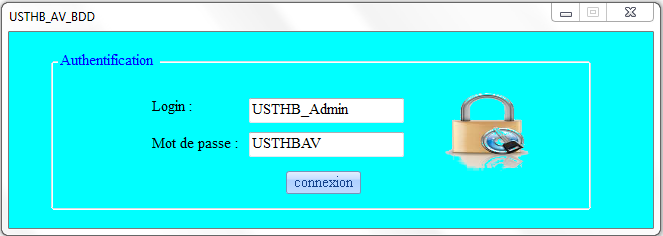
\includegraphics[scale=0.6]{Figures/auth.png}
\caption{L'authentification}
\label{fig :auth} 
\end{center}
\end{figure}

La gestion de la base de signatures permet d'afficher, modifier et supprimer une signature, ainsi que de créer le fichier "info.txt", la figure~\ref{fig :acc} représente la page d'accueil avec  trois fonctionnalités à savoir, la gestion de la base de fichiers légitimes et la gestion de signatures virales et la génération du fichier "info.txt".
\begin{figure}[H]
\begin{center}
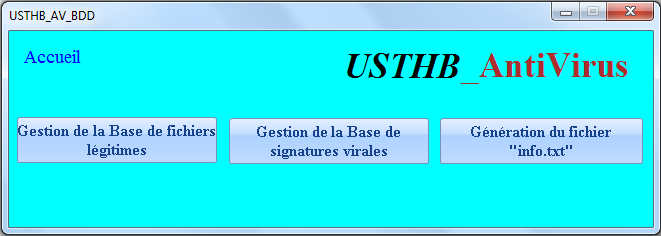
\includegraphics[scale=0.6]{Figures/acc.png}
\caption{La page d'accueil de l'outil de gestion de la base de signatures.}
\label{fig :acc} 
\end{center}
\end{figure}

\subsection{Gestion de la base de fichiers légitimes}
La gestion de la base de fichiers légitimes est composée de deux fonctionnalités :

\subsubsection{Base de fichiers légitimes}
Cette fonctionnalité permet d'afficher la base de fichiers légitimes ainsi que sa taille, la figure~\ref{fig :im3} suivante correspond à une base de 4140 fichiers légitimes.
\begin{figure}[H]
\begin{center}
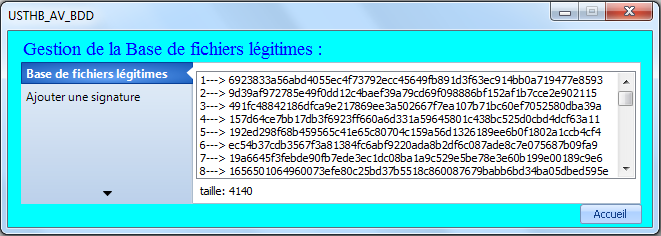
\includegraphics[scale=0.7]{Figures/im3.png}
\caption{La page de la base de fichiers légitimes.}
\label{fig :im3} 
\end{center}
\end{figure}

\subsubsection{Ajouter une signature}
Pour la mise à jour de la base de signatures, l'administrateur peut ajouter une nouvelle signature en suivant les étapes suivantes :\\
\begin{itemize}
\item Sélectionner le fichier légitime à signer en appuyant sur le bouton " … ", qui sera suivi par l'affichage du chemin de fichier sélectionné dans le champ de saisie.
\item Un clic  sur le bouton "ajouter" permet d'insérer le fichier sélectionné dans la base de fichiers légitimes (Figure~\ref{fig :im5})
\end{itemize}
\begin{figure}[H]
\begin{center}
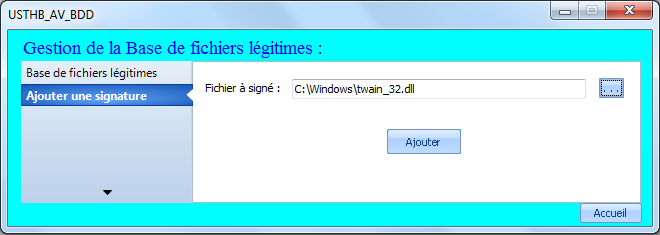
\includegraphics[scale=0.7]{Figures/im5.png}
\caption{La page d'ajouter un fichier légitime.}
\label{fig :im5} 
\end{center}
\end{figure}


\subsection{Gestion de la base de signatures virales}
La gestion de la base de signatures virales est composée de quatre fonctionnalités : 

\subsubsection{Base de malwares} 
Cette fonctionnalité permet d'afficher la base de malwares ainsi que sa taille, la figure~\ref{fig :im12} correspond à une base de 7404 malwares.
\begin{figure}[H]
\begin{center}
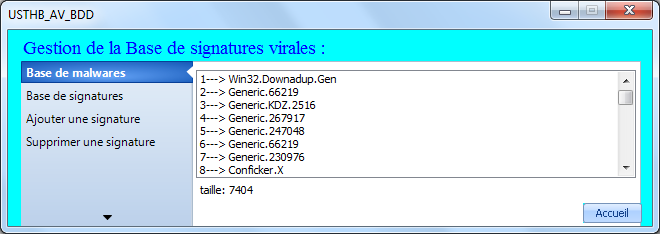
\includegraphics[scale=0.7]{Figures/im12.png}
\caption{La base de malwares.}
\label{fig :im12} 
\end{center}
\end{figure}

\subsubsection{Base de signatures virales}
Cette fonctionnalité permet d'afficher la base de signatures virales, ainsi que sa taille, la figure~\ref{fig :im14} représente une base de 7325 signatures virales :
\begin{figure}[H]
\begin{center}
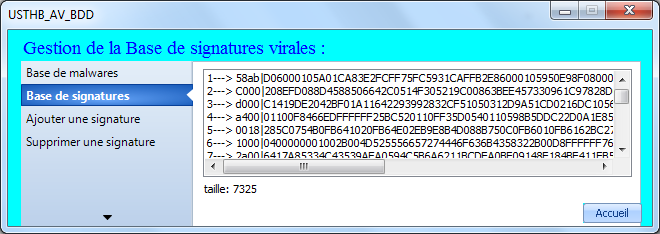
\includegraphics[scale=0.7]{Figures/im14.png}
\caption{La base de signatures virales.}
\label{fig :im14} 
\end{center}
\end{figure}
\subsubsection{Ajouter une signature}
Comme nous avons cité dans le chapitre précédent, une signature virale est composée de quatre champs : un offset, une suite hexadécimale, nom et type de malware, pour ajouter une signature, nous devons suivre les étapes suivantes :
\begin{itemize}
\item Sélectionner le malware à signer avec le bouton "..."
\item Définir l'offset de la suite hexadécimale
\item Récupérer la suite hexadécimale avec le bouton "Récupérer la suite hexadécimale"
\item Définir un nom qui n'existe pas déjà dans la base de signature virale pour ce malware.
\item Définir le type de ce malware 
\item Cliquer sur le bouton "ajouter" pour ajouter la nouvelle signature (Figure~\ref{fig :im7}).      
\end{itemize}
\begin{figure}[H]
\begin{center}
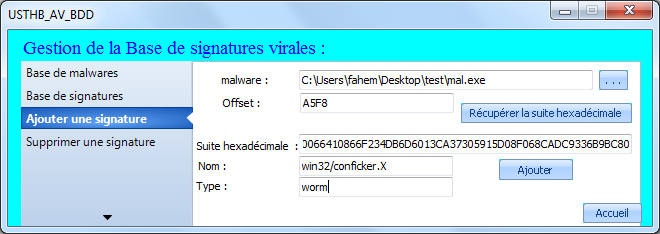
\includegraphics[scale=0.7]{Figures/im7.png}
\caption{Ajouter une signature virale.}
\label{fig :im7} 
\end{center}
\end{figure}

\subsubsection{Supprimer  une signature}
La suppression d'une signature virale nécessite d'indiquer le nom du malware,
dont la signature à supprimer, cette opération s'effectue en deux phases :
\begin{itemize}

\item Saisir le nom du malware 
\item Valider la suppression en cliquant sur bouton "supprimer"(Figure~\ref{fig :im8}).

\end{itemize}
\begin{figure}[H]
\begin{center}
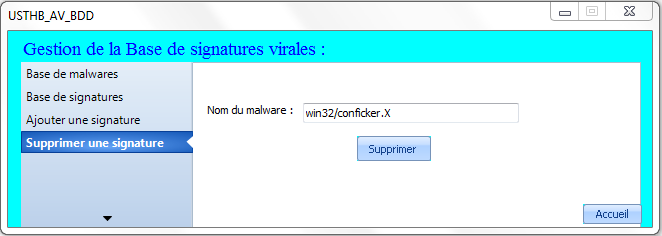
\includegraphics[scale=0.7]{Figures/im8.png}
\caption{Supprimer une signature virale.}
\label{fig :im8} 
\end{center}
\end{figure}
\subsection{Génération du fichier "info.txt"}
Pour créer le fichier "info.txt" l'administrateur doit cliquer sur le bouton "Génération du fichier "info.txt" de la page d'accueil, une fenêtre, contenant des renseignements devant être mis à jour concernant la version de la base de signatures et la version de moteur,s'affiche puis valider par un clic sur le bouton "Générer le fichier" (Figure~\ref{fig :im10}).
\begin{figure}[H]
\begin{center}
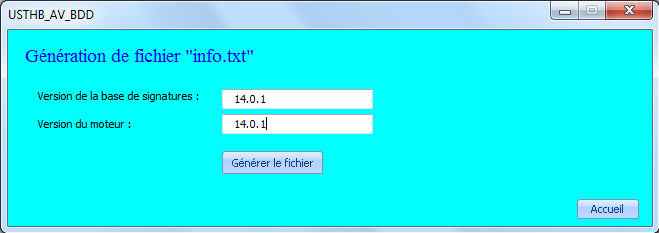
\includegraphics[scale=0.7]{Figures/im10.png}
\caption{Génération du fichier "info.txt".}
\label{fig :im10} 
\end{center}
\end{figure}
\section{Antivirus}

Dans cette partie, nous allons présenter le fonctionnement de notre antivirus.
\subsection{Page d'accueil} 
Dès que l'utilisateur exécute l'antivirus, une page d'accueil sera affichée (Figure~\ref{fig :ant1}), portant les informations et les fonctionnalités suivantes :\\
\begin{itemize}
\item \textbf{Les informations :}
\begin{list}{•}{}
\item Le nom de l'antivirus ( USTHB\_ AntiVirus)
\item L'état actuel de l'antivirus relatif à la dernière mise à jour,dernière analyse, et la version courante de l'antivirus.
\end{list} 
\item \textbf{Les fonctionnalités :}
\begin{list}{•}{}
\item La langue : L'utilisateur coche la langue à utiliser
\item Deux boutons, l'un pour réduire la fenêtre et l'autre pour la fermer
\item Une barre de tâches composée de cinq raccourcis :
\begin{itemize}

\item \textbf{Gestionnaire des tâches : }sert à afficher les programmes, les processus et les services en cours d'exécution sur l'ordinateur et surveiller les performances de l'ordinateur ou pour fermer un programme
\item \textbf{Aide : }permet l'accès au guide d'utilisation
\item \textbf{Exit : }permet de quitter le programme
\item \textbf{Accès internet : }permet un accès rapide sur l'Internet
\item \textbf{Commande cmd : }une fonctionnalité qui offre un point d'entrée pour la saisie de commande Windows.
\end{itemize}
\item Sur la gauche de la page d'accueil, se trouve une barre verticale dont le clic fait apparaitre le menu de l'antivirus.\\
\end{list}
\end{itemize}
La figure~\ref{fig :ant1} montre la page d'accueil de l'antivirus :
\begin{figure}[H]
\begin{center}
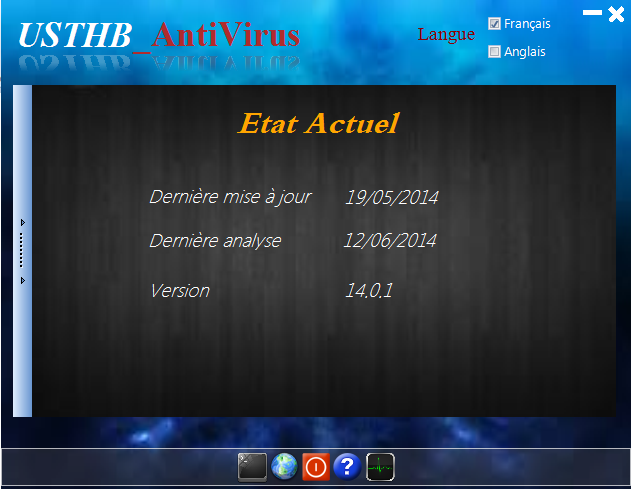
\includegraphics[width=13cm, height=8cm]{Figures/ant1.png}
\caption{Page d'accueil de l'antivirus .}
\label{fig :ant1} 
\end{center}
\end{figure}
\subsection{Page Menu}
Nous trouvons dans cette page les tâches principales de l'antivirus, listées comme suit : Antivirus, Parseur PE, Maintenance, USTHB\_AV, Fichier suspect et protection.\\
La figure~\ref{fig :ant6} montre la page Menu de l'antivirus :
\begin{figure}[H]
\begin{center}
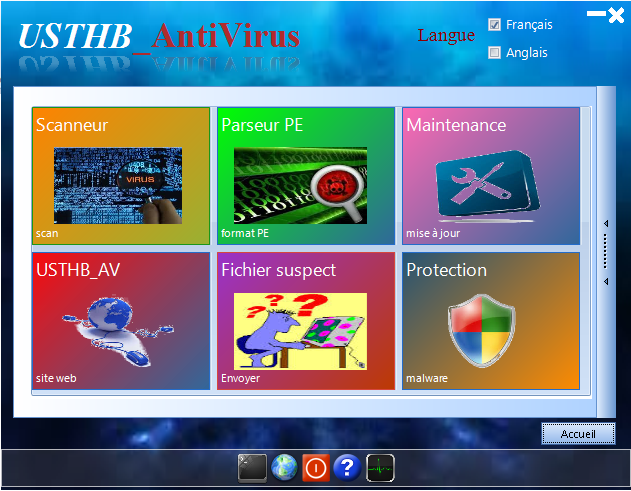
\includegraphics[width=13cm, height=8cm]{Figures/ant6.png}
\caption{Page Menu de l'antivirus .}
\label{fig :ant6} 
\end{center}
\end{figure}
\subsubsection{Scanneur}
L'utilisateur clic sur le champ "Scanneur" pour lancer un scan, une nouvelle page sera affichée(figure~\ref{fig :ant3}), qui contient les quatre types de scan, à savoir ; scan un dossier sélectionné, scan un seul fichier, scan rapide, et scan tout le système.\\
\begin{figure}[H]
\begin{center}
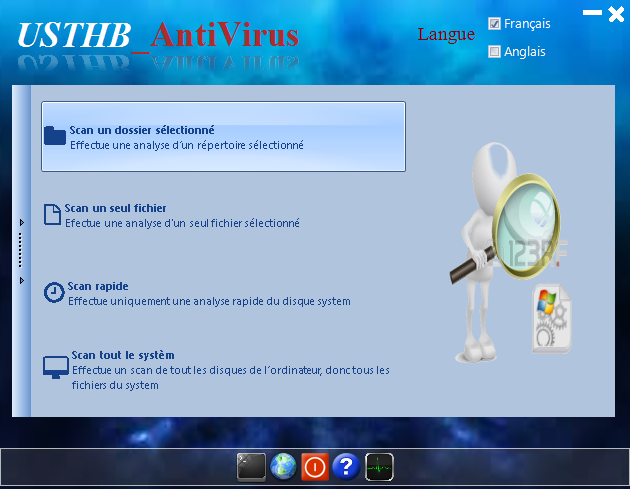
\includegraphics[width=13cm, height=8cm]{Figures/ant3.png}
\caption{Les scans .}
\label{fig :ant3} 
\end{center}
\end{figure}
Selon l'action souhaitable l'utilisateur choisie une des fonctionnalités suivantes :\\

\textit{\textbf{Scan un seul fichier :}}
\begin{list}{•}{}
\item \textbf{Fonctionnement :}\\
Ce champ est choisi une fois le scan aura été pour un seul fichier, le clic sur "scan un seul fichier"  permet d'accéder au chemin de ce fichier, après validation (par un clic sur le bouton OK) le chemin est déclaré dans le champ "fichier analysé".\\
Une fois l'analyse est achevée, trois situations possibles se présentent :\\
\begin{itemize}
\item Le fichier testé est un fichier légitime : un message "le fichier est légitime" est affiché
\item Le fichier testé n'est pas un malware un message "le fichier n'est pan un malware" est affiché
\item Le fichier testé est un malware, dans ce cas, des informations suivantes sont affichées :
\begin{list}{*}{}
\item Le type de malware détecté
\item Une image relative à ce type de malware
\item Une sonnerie d'alerte 
\item Un lien vers la page des résultats d'analyse.\\
\end{list} 
\end{itemize}

La figure~\ref{fig :im14} représente un test d'un fichier "adobe.exe" : \\
\begin{figure}[H]
\begin{center}
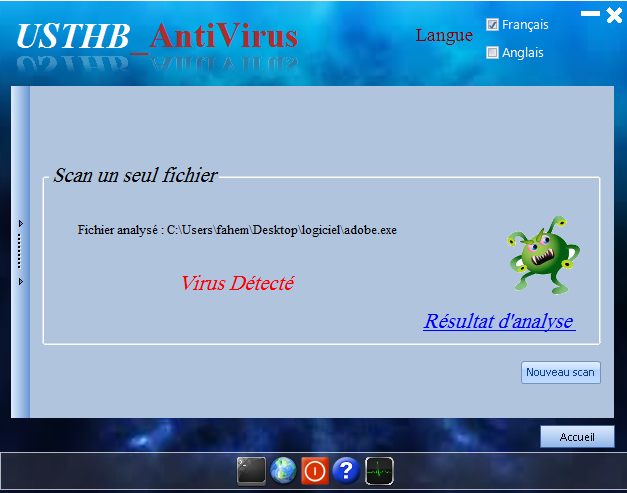
\includegraphics[width=13cm, height=8cm]{Figures/ant14.png}
\caption{Un virus détecté .}
\label{fig :ant6} 
\end{center}
\end{figure}
  
L'utilisateur peut abandonner ou lancer un  nouveau scan par un clic sur le bouton "Nouveau scan", ou visualiser les résultats d'analyse par un clic sur le lien "Résultats d'analyse".
\item \textbf{Résultat d'analyse :}
Après un clic sur le lien "Résultats d'analyse", ces résultats s'affichent dans une nouvelle page, ainsi que les actions qui peuvent être appliquées à ce malware, à savoir ; supprimer, mettre en quarantaine, et ne rien faire, la figure~\ref{fig :ant11} correspond aux résultats d'analyse du fichier "adobe.exe".\\
\begin{figure}[H]
\begin{center}
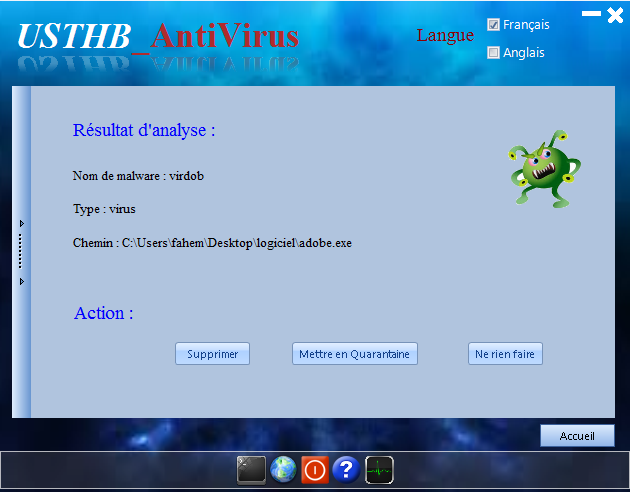
\includegraphics[width=13cm, height=8cm]{Figures/ant11.png}
\caption{L'affichage des résultats d'analyse .}
\label{fig :ant11} 
\end{center}
\end{figure}
\end{list}

\textit{\textbf{Scan un dossier sélectionné : }}
\begin{list}{•}{}
\item \textbf{Fonctionnement : }\\
Ce champ est choisi une fois le dossier à scanner est bien précis, le clic sur "scan un dossier sélectionné"  fait apparaitre une nouvelle page (figure)\\
\begin{itemize}
\item Le dossier à scanner est sélectionné en cliquant sur le bouton " … " cette action permet un accès au chemin de ce dossier 
\item après validation (par un clic sur le bouton OK) le chemin est déclaré dans le champ "répertoire analysé"
\item Au cours de l'analyse des informations ponctuelles vont s'afficher à savoir:
\begin{list}{*}{}
\item Une barre de progression : déclare le taux d'avancement de l'opération
\item Fichier examiné : dans ce champ s'affiche le chemin du fichier en cours d'analyse
\item Temps d'analyse : dans ce champ s'affiche le temps écoulé depuis le début d'analyse
\item Nombre totale : dans ce champ s'affiche le nombre total des fichiers à analyser
\item Malware détecté : dans ce champ s'affiche le nombre final des malwares détectés.
\end{list}

\item A  tout moment l'utilisateur peut effectuer un nouveau type de scan par un simple clic sur le bouton "nouveau scan" qui permet le retour à la page scanneur ou retourner carrément à la page d'accueil  par le bouton "accueil" 
\item Une fois l'analyse est achevée, deux situations possibles se présentent :
\begin{list}{*}{}

\item Aucun malware n'est détecté : un message signalant l'absence des malwares s'affiche 
\item Présence des malwares : une sonnerie d’alerte est déclenchée, signalant la présence de ces malwares, le nombre de ces derniers sera communiqué dans le champ " malware détecté", un nouveau bouton "Résultat d'analyse" sera affiché, pour accéder à ces résultats, il suffit de cliquer sur ce bouton.\\
\end{list}
\end{itemize}
La figure correspond à une analyse d'un dossier nommé logiciel, dont le chemin est \url{C:\User\fahem\Desktop\logiciel}, le résultat de l'analyse est :\\

\begin{itemize}
\item Dernier fichier examiné nommé adobe.exe
\item Temps d'analyse : 0 :01 :47
\item Nombre total : 12
\item Malware détecté : 3

\end{itemize}
\begin{figure}[H]
\begin{center}
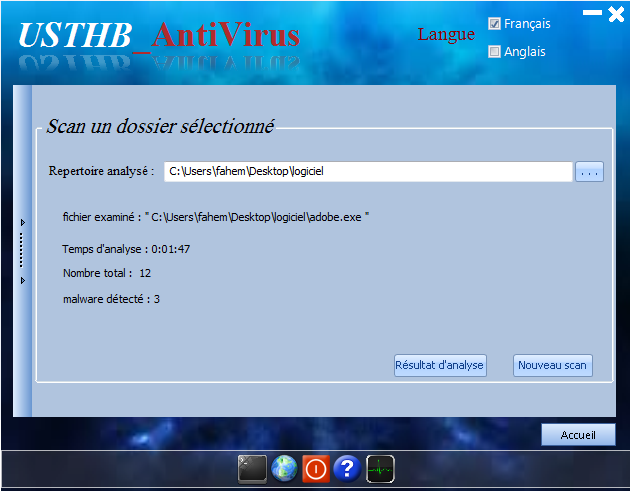
\includegraphics[width=13cm, height=8cm]{Figures/ant13.png}
\caption{Scan un dossier sélectionné .}
\label{fig :ant13} 
\end{center}
\end{figure}
\item \textbf{Résultat d'analyse : }\\
Après un clic sur le bouton "résultat d'analyse", les résultats s'affichent dans une grille, avec deux choix de traitement :\\
\begin{itemize}
\item La suppression ou la mise en quarantaine des malwares un par un, et ce, comme suit :
sélectionner le malware à supprimer ou à  mettre en quarantaine, après on valide l'action par le bouton "Supprimer" ou "mettre en quarantaine", si l'action choisie est faisable, le malware ne s'affiche plus dans la grille, et vis versa  

\item Une action collective  de traitement  pour tous les malwares détectés, à savoir ; supprimer,  mettre en quarantaine, ou ne rien faire, qui sera choisie dans le  CombBox, suivie d'une validation par le bouton "Appliquer".\\
\end{itemize}


Le bouton "Quitter" permet d'abandonner les résultats d'analyse, et un retour automatique  à la page antivirus(Figure~\ref{fig :ant12}).\\
\end{list}
\begin{figure}[H]
\begin{center}
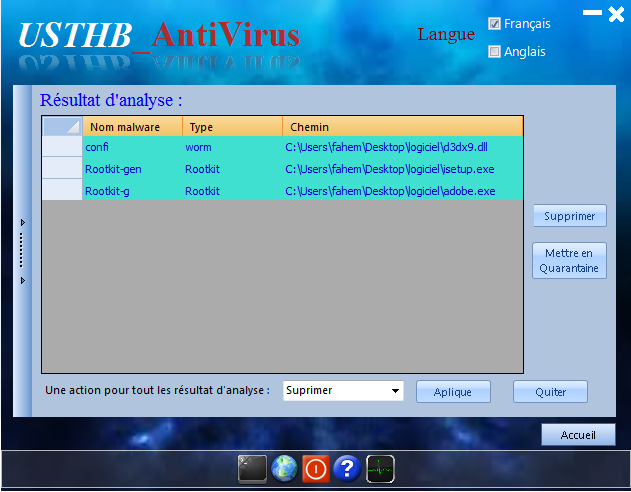
\includegraphics[width=13cm, height=8cm]{Figures/ant12.png}
\caption{Résultats d'analyse d'un dossier sélectionné .}
\label{fig :ant12} 
\end{center}
\end{figure}
\textit{\textbf{Scan rapide : }}\\

Le fonctionnement de ce scan est le même que le scan d'un dossier sélectionné, sauf que la cible d'analyse dans le scan rapide est prédéfinie "C:\", contrairement au scan d'un dossier sélectionné ou l'utilisateur doit sélectionner la cible d'analyse.\\

        
Le traitement des résultats d'analyse dans le scan rapide est basé sur les mêmes principes de scan d'un dossier sélectionné.\\
\textit{\textbf{Scan tout le système }}\\

Le fonctionnement et le traitement des  résultats de ce scan sont les mêmes que le scan rapide, sauf que dans le scan de tout le système, l'ensemble des disques de l'ordinateur seront analysés.

\subsubsection{Parseur PE}

Pour observer le contenu d'un fichier exécutable, l'utilisateur clique sur le champ "Parseur PE" de la page Menu, une nouvelle page apparait, ensuite l'utilisateur doit cliquer sur le bouton " … "   afin d'accéder au chemin du fichier à analyser, après validation (par un clic sur le bouton OK) le chemin est déclaré dans le champ "fichier à analyser", deux cas possibles ont été constatés :\\

\begin{list}{•}{}
\item Le fichier analysé à un format PE non valide : un message "Format PE non valide"
\item Le fichier analysé à un format PE valide : les résultats ; EntryPoint, PE détail, les sections PE,  la liste des fonctions API importées et les éventuels packers utilisés 
seront affichés dans un nouveau champ.\\
\end{list}
La figure~\ref{fig :ant7} représente les résultats d'analyse d'un fichier PE valide :
\begin{figure}[H]
\begin{center}
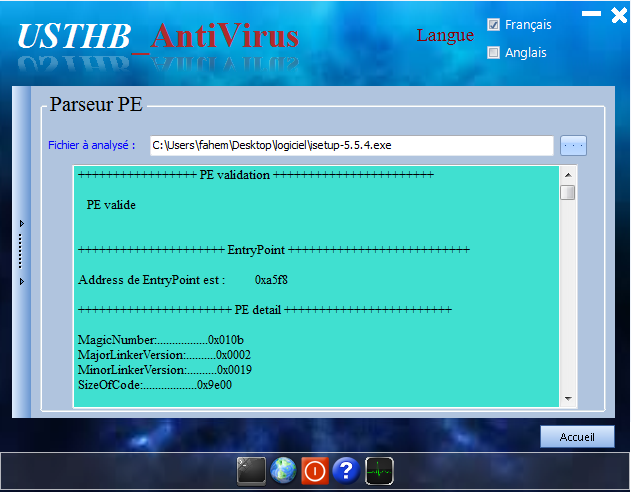
\includegraphics[width=13cm, height=8cm]{Figures/ant7.png}
\caption{Le parseur PE de l'antivirus .}
\label{fig :ant7} 
\end{center}
\end{figure}

\subsubsection{Maintenance}
Pour effectuer une mise à jour, l'utilisateur doit cliquer sur le champ "Maintenance" de la page menu, cette action va faire apparaitre une nouvelle page (Figure) comportant :\\

\begin{list}{•}{}
\item Deux boutons, le premier intitulé "mise à jour de la base de signatures"  le deuxième "mise à jour du programme"
\item Des renseignements concernant la version actuelle de la base de signatures et de programme ainsi que le nombre de signatures
\item Un message encourageant la mise à jour.\\
\end{list}
La mise à jour se déroule par un clic sur l'un des boutons cités précédemment, deux cas sont possibles :\\
\begin{list}{•}{}
\item Il n'existe pas une nouvelle mise à jour : dans ce cas un message "votre antivirus est déjà mis à jour" est affiché
\item Il existe une mise à jour : une barre de progression, qui déclare le taux d'avancement de l'opération, une fois cette dernière est terminée, un message "mise à jour effectuée avec succès" est affiché, en cas d'échec, ce dernier sera déclaré via un message. \\
\end{list}
La figure~\ref{fig :ant5} présente la page de mise à jour de l'antivirus :
\begin{figure}[H]
\begin{center}
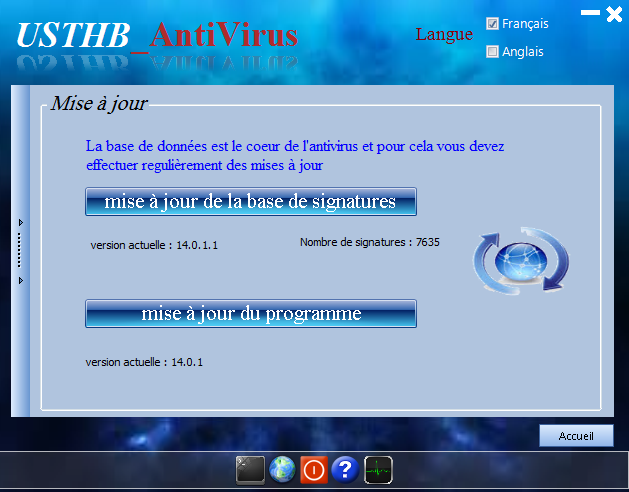
\includegraphics[width=13cm, height=8cm]{Figures/ant5.png}
\caption{La mise à jour de l'antivirus .}
\label{fig :ant5} 
\end{center}
\end{figure}
\subsubsection{USTHB\_AV} 
Pour avoir les dernières actualités sur l'antivirus, télécharger le fichier d'installation de l'antivirus, guide d'utilisation,...\\
L'utilisateur doit cliquer sur le champ "USTHB\_AV" de la page Menu,  cette action permet à l'utilisateur d'accéder au site web de l'antivirus \url{http://usthbav.jimdo.com/}(Figure~\ref{fig :ant2}):
\begin{figure}[H]
\begin{center}
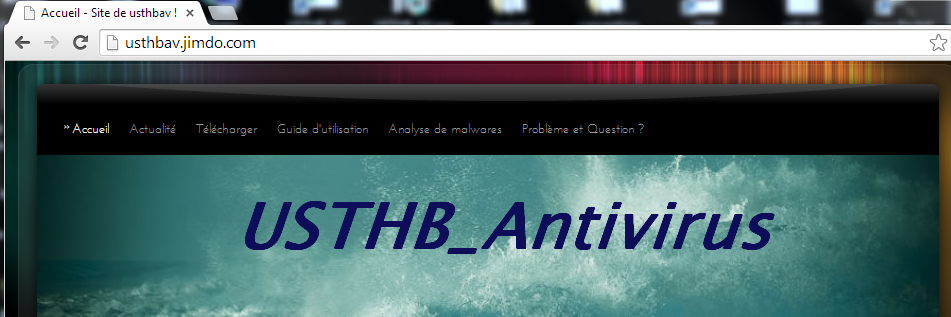
\includegraphics[width=16cm, height=6cm]{Figures/web.png}
\caption{Le site web de l'antivirus .}
\label{fig :ant2} 
\end{center}
\end{figure}
\subsubsection{Fichier suspect}
Pour envoyer un fichier suspect, l'utilisateur doit cliquer sur le champ "Fichier suspect" de la page Menu, cette action va faire apparaitre une nouvelle page (Figure) portant un message décrit les étapes obligatoires à suivre pour envoyer un fichier suspect, qui sont :\\
\begin{list}{•}{}

\item Archiver le fichier suspect à envoyer en ".rar"
\item Définir un mot de passe pour le fichier archivé
\item Cliquer sur le bouton " … "   afin d'accéder au chemin du fichier suspect à envoyer, après validation (par un clic sur le bouton OK) le chemin est déclaré dans le champ "fichier à envoyer"
\item Décrire le fichier suspect au niveau de champ "Sujet" 
\item Accompagner le fichier archivé par le mot de passe de décompression, au niveau de champ "mot de passe de décompression"   
\item Valider l'envoi du fichier suspect par un clic sur le bouton "Envoyer".\\
\end{list}
Après la validation de l'envoi du fichier suspect, une barre de progression sera affichée,  une fois cette dernière est terminée, un message "Fichier envoyé avec succès" est affiché, en cas d'échec, ce dernier sera déclaré via un message.\\

La figure~\ref{fig :ant4} décrit l'envoi d'un fichier suspect, nommé "suspect.rar",  sujet "fichier suspect" et un mot de passe de décompression "Ss000000".
\begin{figure}[H]
\begin{center}
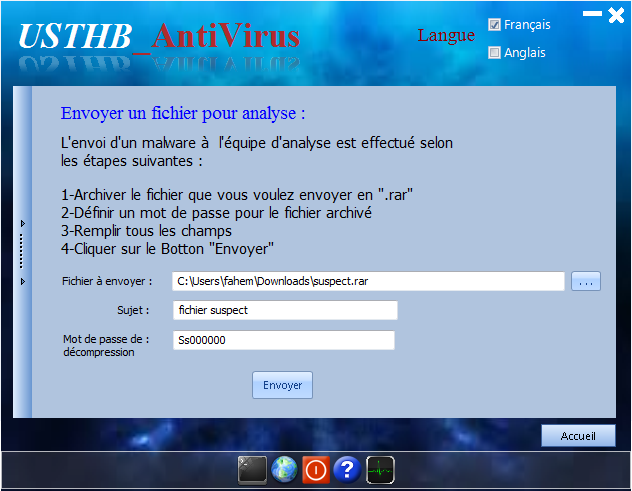
\includegraphics[width=13cm, height=8cm]{Figures/ant4.png}
\caption{L'envoie d'un fichier suspect .}
\label{fig :ant4} 
\end{center}
\end{figure}

\subsubsection{Protection} 
Pour visualiser les informations relatives à l'antivirus, l'utilisateur doit cliquer sur le champ "Protection" de la page Menu, cette action va faire apparaitre une nouvelle page,  portant trois paramètres, détection, informations et quarantaine, indiqué ci- dessous :\\

\begin{list}{•}{}
\item \textbf{Détection : } permet à l'utilisateur de voir la liste des malwares classée par leur nom et type, détectés par l'antivirus(Figure~\ref{fig :ant8})
\begin{figure}[H]
\begin{center}
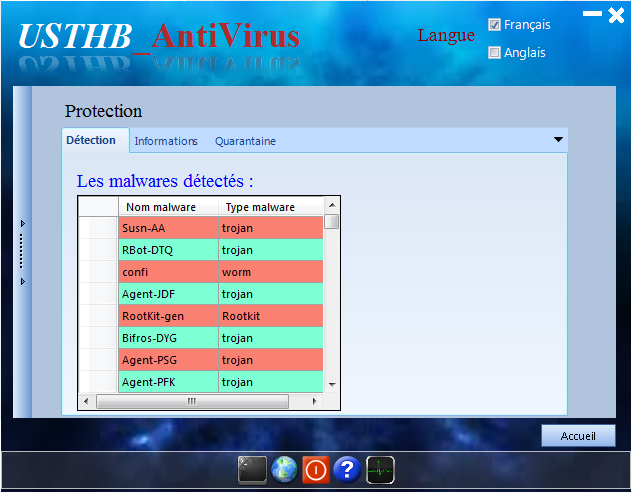
\includegraphics[width=13cm, height=8cm]{Figures/ant8.png}
\caption{Les malwares détectés par l'antivirus .}
\label{fig :ant8} 
\end{center}
\end{figure}
\item \textbf{Information : }Cette partie sert à indiquer les informations relatives à la version actuelle de l'antivirus, qui sont : version de la base virale, nombre de signatures, nombre de malwares détectés et la version du moteur (Figure~\ref{fig :ant9})
\begin{figure}[H]
\begin{center}
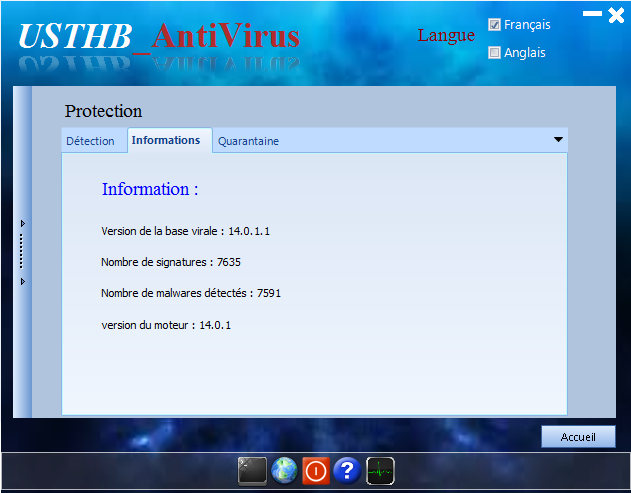
\includegraphics[width=13cm, height=8cm]{Figures/ant9.png}
\caption{Les informations relatives à l'antivirus .}
\label{fig :ant9} 
\end{center}
\end{figure}
\item \textbf{Quarantaine : }Cette option permet à l'utilisateur de visualiser la liste des malwares, déjà mis en quarantaine, la figure~\ref{fig :ant10} représente une quarantaine de trois malwares.  
\begin{figure}[H]
\begin{center}
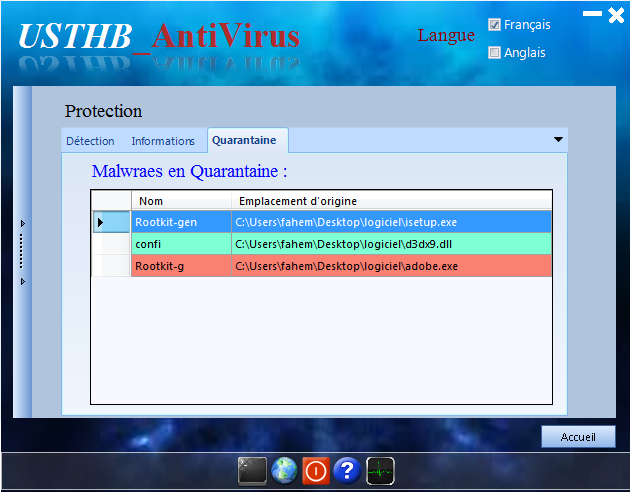
\includegraphics[width=13cm, height=8cm]{Figures/ant10.png}
\caption{Quarantaine .}
\label{fig :ant10} 
\end{center}
\end{figure}
\end{list}
\section{L'accès à l'interface de l'antivirus}
L'utilisateur peut accéder a l'antivirus via trois méthodes différentes :\\
\begin{list}{•}{}

\item \textbf{A partir du Menu démarrer : }la figure~\ref{fig :demar} présente l'apparence de l'antivirus dans le Menu démarrer.
\begin{figure}[H]
\begin{center}
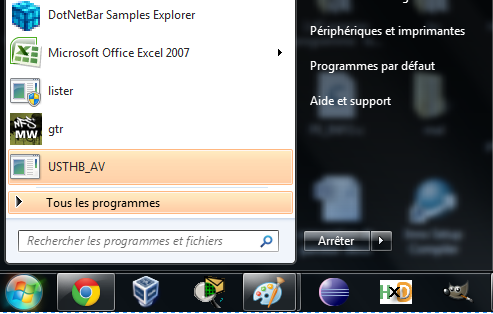
\includegraphics[width=11cm, height=6cm]{Figures/demar.png}
\caption{Menu démarrer.}
\label{fig :demar} 
\end{center}
\end{figure}

\item \textbf{A partir d'un raccourci : }voir la figure~\ref{fig :racc}
\begin{figure}[H]
\begin{center}
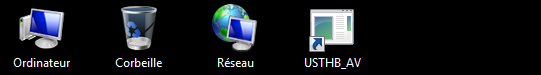
\includegraphics[width=11cm, height=1.5cm]{Figures/racc.png}
\caption{Raccourci au Bureau.}
\label{fig :racc} 
\end{center}
\end{figure}
\item \textbf{A partir de la zone de notification : } la figure~\ref{fig :systray} représente l'apparence de notre antivirus au niveau de la zone de notification ainsi que les tâches que l'on peut effectuer depuis cette zone.
\begin{figure}[H]
\begin{center}
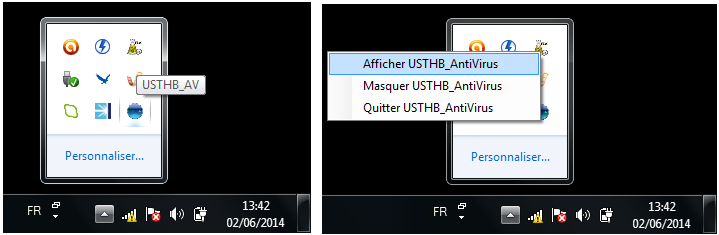
\includegraphics[width=13cm, height=4cm]{Figures/systray.png}
\caption{Zone de notification "Systray".}
\label{fig :systray} 
\end{center}
\end{figure}
\end{list}
\subsection*{Lancement de l'antivirus au démarrage de Windows}
La figure~\ref{fig :run} représente la liste des programmes à lancer au démarrage de Windows
\begin{figure}[H]
\begin{center}
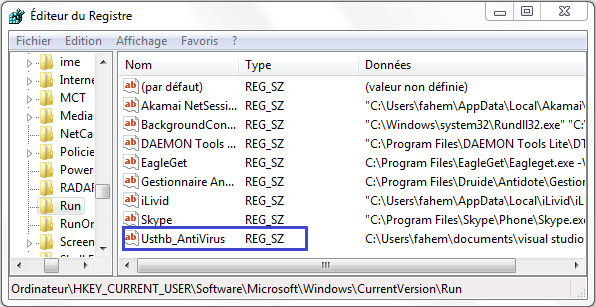
\includegraphics[width=10cm, height=5cm]{Figures/run.png}
\caption{Lancement de l'antivirus au démarrage de windows.}
\label{fig :run} 
\end{center}
\end{figure}
\section{Conclusion}
Dans ce chapitre nous avons vu l'ensemble de fonctionnalités de l'antivirus, côté administrateur "gestion de la base de signatures", côté utilisateur "antivirus". \\

Puis, à travers les impressions écrans, nous avons vu les interfaces, de l'application, illustrant chacune une fonctionnalité. 
